
\chapter{PID Control: The Workhorse}

\begin{quote}
\textit{``The PID controller is arguably the most important control algorithm ever developed. Its simplicity, robustness, and effectiveness have made it the dominant control strategy in industry for nearly a century.''}
\begin{flushright}
--- Karl Johan \r{A}str\"om, \textit{PID Controllers: Theory, Design, and Tuning}
\end{flushright}
\end{quote}

\vspace{1em}

\noindent In this chapter, we explore the Proportional-Integral-Derivative (PID) controller, a control algorithm so successful that it forms the backbone of more than 90\% of all industrial control loops. From the thermostat in your home to the cruise control in your car, from chemical processing plants to spacecraft attitude control, PID controllers are everywhere. We will trace the historical development of this remarkable algorithm, develop its mathematical foundation rigorously, and build practical intuition through hands-on experiments.

%=============================================================================
\section{Historical Development: From Ship Steering to Industrial Standard}
%=============================================================================

The story of PID control is fundamentally a story of practical engineering challenges driving theoretical development. Unlike many control concepts that emerged from academic research, PID control arose from the urgent need to automate steering of ships, and its theory was developed largely to explain what clever engineers had already built.

\subsection{Elmer Sperry and the Dawn of Automatic Control (1911)}

The year 1911 marked a turning point in the history of automatic control. Elmer Ambrose Sperry, an American inventor and entrepreneur who had already made significant contributions to electric lighting and mining equipment, turned his attention to the problem of ship stabilization and steering.

Ships of the early 20th century faced a fundamental control challenge. A helmsman steering a large vessel must constantly counteract the effects of waves, currents, and wind. This is exhausting work, and human operators are prone to fatigue and inconsistency. Sperry recognized that the gyroscope---a device he had been perfecting for years---could sense a ship's deviation from course, and this information could be used to automatically adjust the rudder.

Sperry's \textbf{gyroscopic ship stabilizer}, patented in 1908 and first tested on the USS Worden in 1911, represented one of the earliest practical applications of proportional control. The fundamental principle was elegant: the gyroscope detected the ship's angular deviation from the desired heading, and this error signal was amplified and used to drive the rudder in the opposite direction.

Mathematically, Sperry's system implemented what we now call \textbf{proportional control}:
\begin{equation}
\delta(t) = \Kp \cdot e(t)
\label{eq:proportional_basic}
\end{equation}
where $\delta(t)$ is the rudder angle, $e(t) = \theta_{\text{desired}} - \theta_{\text{actual}}$ is the heading error, and $\Kp$ is the proportional gain.

The system worked remarkably well under many conditions, but Sperry and his engineers soon encountered a frustrating phenomenon. When ocean currents or steady winds pushed the ship off course, the proportional controller would find an equilibrium position where the rudder was deflected just enough to maintain a constant---but non-zero---heading error. This \textbf{steady-state error} was an inherent limitation of proportional-only control, a fact that would take another decade to be fully understood and addressed.

\begin{figure}[htbp]
\centering
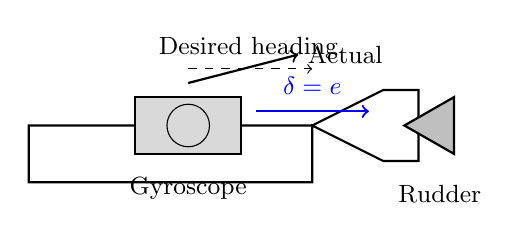
\begin{tikzpicture}[scale=0.9]
    % Ship outline
    \draw[thick] (0,0) -- (4,0) -- (5,0.5) -- (5.5,0.5) -- (5.5,-0.5) -- (5,-0.5) -- (4,0) -- (4,-0.8) -- (0,-0.8) -- cycle;

    % Gyroscope housing
    \draw[thick, fill=gray!30] (1.5,-0.4) rectangle (3,0.4);
    \draw (2.25,0) circle (0.3);
    \node[below] at (2.25,-0.6) {\small Gyroscope};

    % Rudder
    \draw[thick, fill=gray!50] (5.3,0) -- (6,0.4) -- (6,-0.4) -- cycle;
    \node[below] at (5.8,-0.7) {\small Rudder};

    % Error signal arrow
    \draw[->, thick, blue] (3.2,0.2) -- (4.8,0.2);
    \node[above, blue] at (4,0.3) {\small $\delta = \Kp e$};

    % Desired heading
    \draw[->, dashed] (2.25,0.8) -- (4,0.8);
    \node[above] at (3.1,0.8) {\small Desired heading};

    % Actual heading (slightly off)
    \draw[->, thick] (2.25,0.6) -- (3.8,1.0);
    \node[right] at (3.8,1.0) {\small Actual};
\end{tikzpicture}
\caption{Sperry's gyroscopic ship stabilizer (1911) implemented proportional control. The gyroscope detected heading error, which was amplified to drive the rudder.}
\label{fig:sperry_system}
\end{figure}

\subsection{Nicolas Minorsky: The First Theory of PID Control (1922)}

\begin{historicalbox}[Nicolas Minorsky and the Birth of PID Theory]
Nicolas Minorsky (1885--1970), a Russian-American engineer working for the United States Navy, bridged the gap between engineering practice and theoretical understanding. In his landmark 1922 paper, ``Directional Stability of Automatically Steered Bodies,'' published in the \textit{Journal of the American Society of Naval Engineers}, Minorsky provided the first complete theoretical analysis of what we now call PID control. He tested his three-term controller on the USS New Mexico in 1922, demonstrating that the ship could maintain its heading within $\pm 1/6$ of a degree---an unprecedented level of precision for the time.
\end{historicalbox}

Minorsky had been tasked with improving the automatic steering systems used on naval vessels, and he approached the problem with a mathematician's rigor combined with an engineer's practical sensibility. His key insight came from observing how experienced helmsmen steered ships.

Minorsky noted that skilled helmsmen did not simply apply a rudder correction proportional to the current heading error. Instead, they applied a correction proportional to the current error (P action), applied additional correction when the error persisted over time (I action), and anticipated where the ship was heading based on how fast the error was changing (D action). This observation led Minorsky to propose the three-term controller:
\begin{equation}
\delta(t) = \Kp e(t) + \Ki \int_0^t e(\tau) \, d\tau + \Kd \frac{de(t)}{dt}
\label{eq:minorsky_pid}
\end{equation}

Minorsky's analysis was groundbreaking not just for proposing this controller structure, but for providing a mathematical framework to understand why each term was necessary. The \textbf{proportional term} provides the primary corrective action, where larger errors produce larger corrections; however, for a stable equilibrium with non-zero external disturbance, the system must maintain some error to generate the necessary restoring force. The \textbf{integral term} accumulates error over time, so that even a small persistent error will eventually produce a large integral, driving the system to eliminate the steady-state offset---Minorsky recognized this as the key to achieving zero steady-state error. The \textbf{derivative term} responds to the rate of change of error: when the ship is rapidly approaching the desired heading, the derivative term applies a ``braking'' action, reducing overshoot and oscillation.

Minorsky tested his three-term controller on the USS New Mexico in 1922, demonstrating dramatically improved steering performance compared to proportional-only systems. The ship could maintain its heading within $\pm 1/6$ of a degree---an unprecedented level of precision for the time.

\subsection{The Industrial Revolution in Control: Pneumatic PID (1930s--1940s)}

While Minorsky's work established the theoretical foundation, the widespread adoption of PID control required practical, reliable hardware. The 1930s saw the emergence of \textbf{pneumatic controllers}---devices that used compressed air to implement the mathematical operations of PID control.

The appeal of pneumatic systems was manifold. Compressed air was already widely available in industrial settings, pneumatic devices were inherently safe in explosive atmospheres (no electrical sparks), and the technology was robust and easy to maintain. Most importantly, clever mechanical design could implement the calculus operations---integration and differentiation---using physical principles.

\begin{figure}[htbp]
\centering
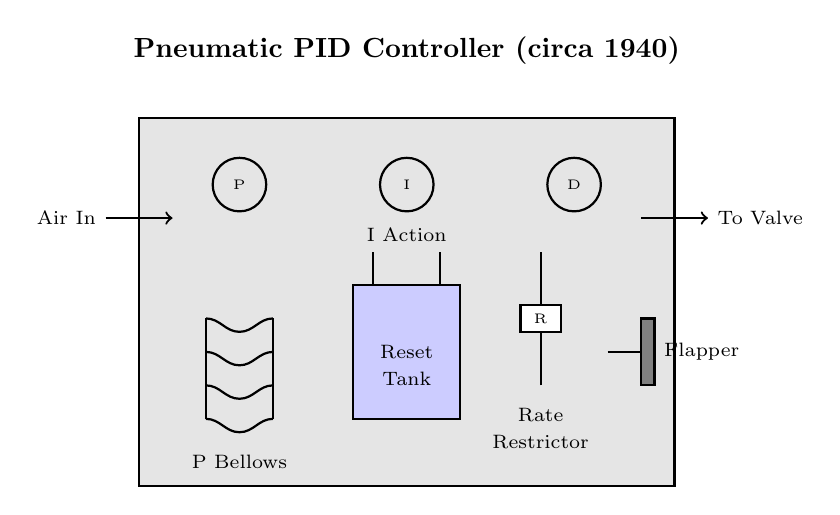
\begin{tikzpicture}[scale=0.85]
    % Title
    \node[font=\bfseries] at (4,6.5) {Pneumatic PID Controller (circa 1940)};

    % Main housing
    \draw[thick, fill=gray!20] (0,0) rectangle (8,5.5);

    % Bellows for P action
    \draw[thick] (1,1) -- (1,2.5);
    \draw[thick] (1,1) to[out=0,in=180] (1.5,0.8) to[out=0,in=180] (2,1);
    \draw[thick] (1,1.5) to[out=0,in=180] (1.5,1.3) to[out=0,in=180] (2,1.5);
    \draw[thick] (1,2) to[out=0,in=180] (1.5,1.8) to[out=0,in=180] (2,2);
    \draw[thick] (1,2.5) to[out=0,in=180] (1.5,2.3) to[out=0,in=180] (2,2.5);
    \draw[thick] (2,1) -- (2,2.5);
    \node[below] at (1.5,0.6) {\scriptsize P Bellows};

    % I action - tank
    \draw[thick, fill=blue!20] (3.2,1) rectangle (4.8,3);
    \node at (4,2) {\scriptsize Reset};
    \node at (4,1.6) {\scriptsize Tank};
    \draw[thick] (3.5,3) -- (3.5,3.5);
    \draw[thick] (4.5,3) -- (4.5,3.5);
    \node[above] at (4,3.5) {\scriptsize I Action};

    % D action - restriction
    \draw[thick] (6,1.5) -- (6,3.5);
    \draw[thick, fill=white] (5.7,2.3) rectangle (6.3,2.7);
    \node at (6,2.5) {\tiny R};
    \node[below] at (6,1.3) {\scriptsize Rate};
    \node[below] at (6,0.9) {\scriptsize Restrictor};

    % Nozzle-flapper
    \draw[thick] (7,2) -- (7.5,2);
    \draw[thick, fill=gray] (7.5,1.5) rectangle (7.7,2.5);
    \node[right] at (7.7,2) {\scriptsize Flapper};

    % Air supply
    \draw[->, thick] (-0.5,4) -- (0.5,4);
    \node[left] at (-0.5,4) {\scriptsize Air In};

    % Output
    \draw[->, thick] (7.5,4) -- (8.5,4);
    \node[right] at (8.5,4) {\scriptsize To Valve};

    % Dials on front
    \draw[thick] (1.5,4.5) circle (0.4);
    \node at (1.5,4.5) {\tiny P};
    \draw[thick] (4,4.5) circle (0.4);
    \node at (4,4.5) {\tiny I};
    \draw[thick] (6.5,4.5) circle (0.4);
    \node at (6.5,4.5) {\tiny D};
\end{tikzpicture}
\caption{Schematic representation of a 1940s pneumatic PID controller. Bellows provided proportional action, a reset tank with restriction provided integral action, and a rate restrictor provided derivative action. Adjustment knobs on the front panel allowed operators to tune each gain.}
\label{fig:pneumatic_pid}
\end{figure}

Two companies led the commercialization of pneumatic PID controllers:

\textbf{Taylor Instrument Companies} (founded 1851) introduced their Fulscope controller series in the 1930s. These instruments featured a novel ``force-balance'' design where mechanical elements were balanced against spring forces, providing stable and accurate control action. Taylor's controllers became standard equipment in the chemical and petroleum industries.

\textbf{Foxboro Company} (founded 1908) pioneered the use of the ``nozzle-flapper'' mechanism, which converted small mechanical displacements into pneumatic pressure changes. Their Model 40 controller, introduced in 1937, was one of the first commercially successful pneumatic PID controllers and remained in production for decades.

The pneumatic implementation of integral action was particularly ingenious. A bellows connected to a tank through a restrictor valve would slowly fill or empty as the error signal persisted. The time constant of this RC-like pneumatic circuit determined the integral time constant $\Ti$. Derivative action was implemented through similar pneumatic circuits that responded to the rate of pressure change.

\subsection{Why PID Dominates: The 90\% Solution}

Today, surveys consistently show that PID controllers constitute approximately 90--95\% of all control loops in industrial settings. This remarkable dominance is not because PID is optimal---more sophisticated control strategies exist---but because PID offers an unmatched combination of desirable properties. First, PID provides \textbf{simplicity}, as three parameters capture the essential dynamics of most control problems. Second, PID controllers exhibit \textbf{robustness}, tolerating significant model uncertainty without becoming unstable. Third, \textbf{tunability} allows operators to adjust behavior without deep theoretical knowledge. Fourth, \textbf{universality} means the same algorithm works for temperature, pressure, flow, level, speed, and countless other variables. Finally, the \textbf{maturity} of the technology, with nearly a century of engineering experience, has produced reliable tuning methods. As we develop the mathematical theory in subsequent sections, keep in mind that PID's endurance comes not from mathematical elegance alone, but from its practical effectiveness across an enormous range of applications.


%=============================================================================
\section{Modern Applications: PID in the 21st Century}
%=============================================================================

While the mathematical foundation of PID control was established in the 1920s, the algorithm remains as relevant as ever in modern engineering. Digital implementation has made PID controllers more precise, more flexible, and more accessible than their pneumatic predecessors. Let us examine several contemporary applications.

\subsection{HVAC Systems and Smart Thermostats}

The thermostat in your home or office implements PID control to maintain comfortable temperatures. Modern smart thermostats like the Nest or Ecobee use sophisticated digital PID algorithms with additional features. These include \textbf{adaptive tuning}, where the controller learns the thermal characteristics of your building, as well as \textbf{predictive heating/cooling}, which anticipates when to start conditioning based on learned patterns. Additionally, \textbf{anti-windup} mechanisms prevent the integral term from accumulating when heating or cooling is saturated.

A typical home HVAC system might use a PI controller (derivative action is often omitted due to noise sensitivity):
\begin{equation}
u(t) = \Kp \left[ e(t) + \frac{1}{\Ti} \int_0^t e(\tau) \, d\tau \right]
\end{equation}
where $u(t)$ is the heating/cooling command, $e(t) = T_{\text{setpoint}} - T_{\text{measured}}$, and typical values might be $\Kp = 2$--$5$ and $\Ti = 5$--$15$ minutes.

\subsection{Drone Flight Controllers}

Multirotor drones (quadcopters, hexacopters, etc.) rely heavily on PID control for stabilization. A typical drone runs multiple cascaded PID loops at different frequencies. The innermost \textbf{rate controllers} are PID loops controlling angular velocity around the roll, pitch, and yaw axes, running at 1--8 kHz. The \textbf{attitude controllers} form the outer loop, controlling orientation angles at 250--1000 Hz. Finally, \textbf{position controllers} provide PID loops for GPS hold and waypoint navigation, running at 10--50 Hz. The cascaded structure allows each loop to be tuned independently, and the fast inner loops provide stability while the slower outer loops provide trajectory tracking.

\subsection{3D Printer Temperature Control}

Fused deposition modeling (FDM) 3D printers require precise temperature control of both the hot end (extruder) and heated bed. Temperature deviations of even a few degrees can cause print quality issues such as stringing, warping, or poor layer adhesion.

Most 3D printer firmware (Marlin, RepRapFirmware, Klipper) implements PID control for temperature regulation. A typical hot end might use:
\begin{align}
\Kp &\approx 20\text{--}30 \\
\Ki &\approx 1\text{--}3 \\
\Kd &\approx 50\text{--}100
\end{align}

The relatively high derivative gain helps counteract the thermal lag inherent in heating elements, providing faster response to temperature disturbances when filament flow changes.

\subsection{Automotive Engine Management}

Modern vehicles contain dozens of PID control loops managing everything from idle speed to air-fuel ratio to electronic throttle position. The electronic fuel injection system, for example, uses PID control to maintain the stoichiometric air-fuel ratio required for optimal catalytic converter performance. In this system, oxygen sensors measure exhaust composition, and a PID controller adjusts the fuel injector pulse width accordingly. The integral action ensures zero steady-state error in the average air-fuel ratio, while derivative action (often filtered) provides fast transient response.

These automotive PID loops must function reliably across extreme temperature ranges, varying altitudes, and component aging---a testament to the robustness of the PID algorithm.


%=============================================================================
\section{Mathematical Foundation}
%=============================================================================

Having established the historical context and practical importance of PID control, we now develop its mathematical foundation rigorously. This section provides the theoretical tools needed to analyze, design, and tune PID controllers.

\subsection{The PID Control Law}

\begin{definition}[PID Controller]
A \textbf{Proportional-Integral-Derivative (PID) controller} generates a control signal $u(t)$ based on the error signal $e(t) = r(t) - y(t)$, where $r(t)$ is the reference (setpoint) and $y(t)$ is the measured output:
\begin{equation}
\boxed{u(t) = \Kp e(t) + \Ki \int_0^t e(\tau) \, d\tau + \Kd \frac{de(t)}{dt}}
\label{eq:pid_time}
\end{equation}
where $\Kp$ is the proportional gain, $\Ki$ is the integral gain, and $\Kd$ is the derivative gain.
\end{definition}

This is called the \textbf{parallel form} or \textbf{independent gains form} of the PID controller. An alternative \textbf{standard form} (also called \textbf{ideal form} or \textbf{ISA form}) writes:
\begin{equation}
u(t) = \Kp \left[ e(t) + \frac{1}{\Ti} \int_0^t e(\tau) \, d\tau + \Td \frac{de(t)}{dt} \right]
\label{eq:pid_standard}
\end{equation}
where $\Ti = \Kp/\Ki$ is the \textbf{integral time} (or \textbf{reset time}) and $\Td = \Kd/\Kp$ is the \textbf{derivative time} (or \textbf{rate time}).

The relationship between the two forms is:
\begin{equation}
\Ki = \frac{\Kp}{\Ti}, \qquad \Kd = \Kp \Td
\end{equation}

\subsection{Transfer Function Representation}

Taking the Laplace transform of Eq.~\eqref{eq:pid_time} (assuming zero initial conditions):
\begin{align}
U(s) &= \Kp E(s) + \Ki \frac{E(s)}{s} + \Kd s E(s) \\
&= \left( \Kp + \frac{\Ki}{s} + \Kd s \right) E(s)
\end{align}

The \textbf{PID transfer function} is therefore:
\begin{equation}
\boxed{C(s) = \frac{U(s)}{E(s)} = \Kp + \frac{\Ki}{s} + \Kd s}
\label{eq:pid_tf_parallel}
\end{equation}

In the standard form:
\begin{equation}
C(s) = \Kp \left( 1 + \frac{1}{\Ti s} + \Td s \right)
\label{eq:pid_tf_standard}
\end{equation}

Combining terms over a common denominator:
\begin{equation}
C(s) = \frac{\Kd s^2 + \Kp s + \Ki}{s} = \Kp \cdot \frac{\Ti \Td s^2 + \Ti s + 1}{\Ti s}
\label{eq:pid_tf_combined}
\end{equation}

This reveals that the PID controller has one pole at $s = 0$ (from the integral action) and two zeros (from the numerator polynomial). The zeros are located at:
\begin{equation}
s = \frac{-\Kp \pm \sqrt{\Kp^2 - 4\Kd\Ki}}{2\Kd}
\end{equation}

\begin{figure}[htbp]
\centering
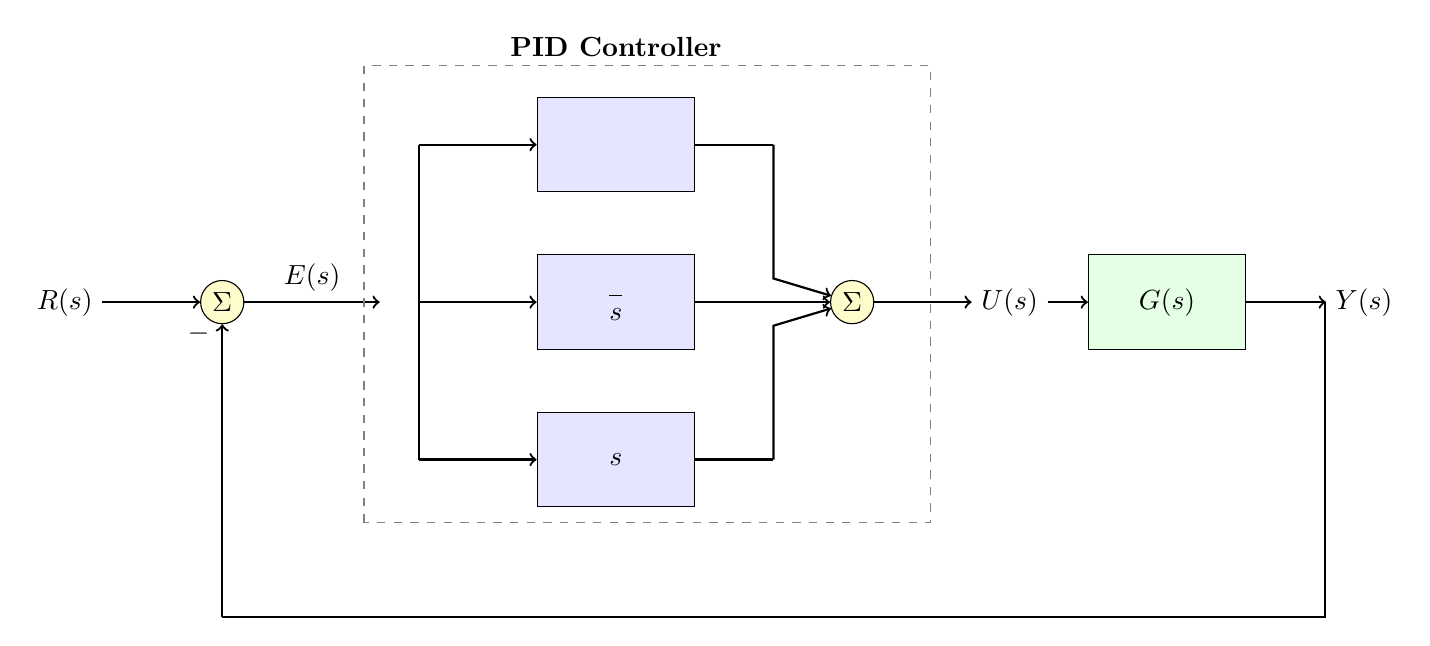
\begin{tikzpicture}[
    block/.style={draw, fill=blue!10, rectangle, minimum height=1.2cm, minimum width=2cm},
    sum/.style={draw, fill=yellow!20, circle, inner sep=2pt},
    arrow/.style={->, thick}
]
    % Input
    \node (r) at (-1,0) {$R(s)$};

    % Sum junction
    \node[sum] (sum1) at (1,0) {$\Sigma$};
    \draw[arrow] (r) -- (sum1);

    % Error signal
    \node (e) at (2.5,0) {};
    \draw[arrow] (sum1) -- node[above] {$E(s)$} (3,0);

    % Branch point
    \coordinate (branch) at (3.5,0);

    % P block
    \node[block] (P) at (6,2) {$\Kp$};

    % I block
    \node[block] (I) at (6,0) {$\displaystyle\frac{\Ki}{s}$};

    % D block
    \node[block] (D) at (6,-2) {$\Kd s$};

    % Connections to blocks
    \draw[thick] (3.5,0) -- (3.5,2);
    \draw[arrow] (3.5,2) -- (P);
    \draw[arrow] (3.5,0) -- (I);
    \draw[thick] (3.5,0) -- (3.5,-2);
    \draw[arrow] (3.5,-2) -- (D);

    % Sum junction 2
    \node[sum] (sum2) at (9,0) {$\Sigma$};

    % Connections from blocks
    \draw[thick] (P) -- (8,2);
    \draw[arrow] (8,2) -- (8,0.3) -- (sum2);
    \draw[arrow] (I) -- (sum2);
    \draw[thick] (D) -- (8,-2);
    \draw[arrow] (8,-2) -- (8,-0.3) -- (sum2);

    % Output
    \node (u) at (11,0) {$U(s)$};
    \draw[arrow] (sum2) -- (u);

    % Plant
    \node[block, fill=green!10] (G) at (13,0) {$G(s)$};
    \draw[arrow] (u) -- (G);

    % Output y
    \node (y) at (15.5,0) {$Y(s)$};
    \draw[arrow] (G) -- (y);

    % Feedback
    \draw[thick] (15,0) -- (15,-4) -- (1,-4);
    \draw[arrow] (1,-4) -- (sum1);
    \node at (0.7,-0.4) {$-$};

    % Labels
    \node[above] at (6,3) {\textbf{PID Controller}};
    \draw[dashed, gray] (2.8,-2.8) rectangle (10,3);
\end{tikzpicture}
\caption{Block diagram of a PID control system in parallel form. The error signal $E(s)$ is processed by three parallel paths: proportional ($\Kp$), integral ($\Ki/s$), and derivative ($\Kd s$). The outputs are summed to produce the control signal $U(s)$.}
\label{fig:pid_block_diagram}
\end{figure}

\subsection{Proportional Action: Fast Response, Persistent Error}

Consider a closed-loop system with proportional-only control $C(s) = \Kp$ and a plant $G(s)$. The closed-loop transfer function is:
\begin{equation}
T(s) = \frac{\Kp G(s)}{1 + \Kp G(s)}
\end{equation}

\textbf{Effect on transient response:} Higher $\Kp$ generally produces faster response (higher bandwidth) but may lead to increased overshoot and oscillation, potentially causing instability.

\textbf{Effect on steady-state error:} For a unit step input $R(s) = 1/s$, the final value theorem gives:
\begin{equation}
e_{ss} = \lim_{s \to 0} s \cdot \frac{1}{1 + \Kp G(s)} \cdot \frac{1}{s} = \frac{1}{1 + \Kp G(0)}
\end{equation}

For a Type 0 system (no free integrators in $G(s)$), we have $G(0) = K_{\text{plant}}$ (the DC gain), so:
\begin{equation}
\boxed{e_{ss} = \frac{1}{1 + \Kp K_{\text{plant}}}}
\label{eq:p_only_error}
\end{equation}

This fundamental result shows that \textbf{proportional control alone cannot eliminate steady-state error for Type 0 plants}. Even with very large $\Kp$, some residual error remains. This was exactly the problem Sperry encountered with his ship autopilot.

\begin{example}[P-Only Control of a First-Order Plant]
Consider a thermal system with transfer function $G(s) = \dfrac{1}{10s + 1}$, representing a time constant of 10 seconds and unity DC gain. A P-only controller with $\Kp = 4$ is used.

\textbf{Closed-loop transfer function:}
\begin{equation*}
T(s) = \frac{4 \cdot \frac{1}{10s+1}}{1 + 4 \cdot \frac{1}{10s+1}} = \frac{4}{10s + 1 + 4} = \frac{4}{10s + 5} = \frac{0.8}{2s + 1}
\end{equation*}

\textbf{Steady-state error to unit step:}
\begin{equation*}
e_{ss} = \frac{1}{1 + 4 \cdot 1} = \frac{1}{5} = 0.2 = 20\%
\end{equation*}

The output reaches only 80\% of the setpoint. To reduce this error to 5\%, we would need:
\begin{equation*}
\frac{1}{1 + \Kp} = 0.05 \implies \Kp = 19
\end{equation*}

But such high gain may cause stability problems in more complex systems.
\end{example}

\subsection{Integral Action: Eliminating Steady-State Error}

The integral term addresses the fundamental limitation of proportional control by accumulating error over time:
\begin{equation}
u_I(t) = \Ki \int_0^t e(\tau) \, d\tau
\end{equation}

Even when the proportional term becomes small (as error decreases), the integral term continues to provide a control effort based on the history of errors. At steady state, the integral term will grow (or shrink) until the error is driven to zero.

\textbf{Mechanism:} Suppose the system reaches a quasi-steady state with $e = e_0 \neq 0$. The integral term grows as $\Ki e_0 t$, continuously increasing the control effort. This pushes the output toward the setpoint. Only when $e = 0$ (on average) does the integral stop accumulating, meaning steady-state error must be zero.

Mathematically, adding an integrator to the controller increases the \textbf{system type} by one. For a PI controller:
\begin{equation}
C(s) = \Kp + \frac{\Ki}{s} = \frac{\Kp s + \Ki}{s}
\end{equation}

The additional pole at $s = 0$ ensures zero steady-state error for step inputs (and zero steady-state error for ramp inputs if the plant already has one integrator).

\begin{remark}[Integral Windup]
A practical issue with integral action is \textbf{integral windup}. When the actuator saturates (e.g., a valve fully open), the integral term continues to accumulate error even though no additional control action is possible. When the error finally reverses, the large accumulated integral causes excessive overshoot and slow recovery. Anti-windup schemes (discussed in Chapter 11) address this problem.
\end{remark}

\subsection{Derivative Action: Anticipation and Damping}

The derivative term responds to the rate of change of error:
\begin{equation}
u_D(t) = \Kd \frac{de(t)}{dt}
\end{equation}

\textbf{Physical interpretation:} If the error is decreasing rapidly (the system is approaching the setpoint quickly), the derivative term applies a ``braking'' force, reducing overshoot. Conversely, if a disturbance is causing the error to grow, the derivative term provides an early corrective response before the proportional term can react significantly.

\textbf{Frequency domain perspective:} The derivative $\Kd s$ has magnitude $|\Kd s| = \Kd \omega$ increasing with frequency. This provides \textbf{phase lead}, where the phase contribution of $+90°$ at all frequencies can improve phase margin, as well as \textbf{increased bandwidth} due to amplified high-frequency response.

\textbf{Noise amplification:} The derivative term is rarely used in its pure form because it amplifies high-frequency measurement noise. A practical solution is the \textbf{filtered derivative}:
\begin{equation}
D(s) = \frac{\Kd s}{1 + \frac{\Kd}{N\Kp} s} = \frac{\Kd s}{1 + \frac{\Td}{N} s}
\label{eq:filtered_derivative}
\end{equation}
where $N$ is typically chosen between 8 and 20. This provides derivative action at lower frequencies while rolling off at higher frequencies.

\begin{figure}[htbp]
\centering
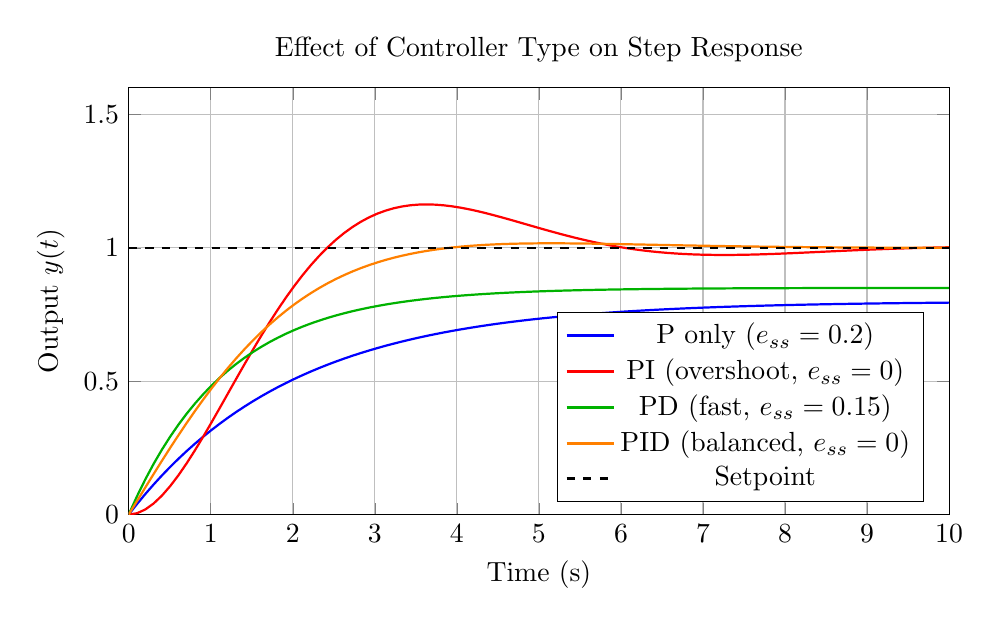
\begin{tikzpicture}
\begin{axis}[
    width=12cm,
    height=7cm,
    xlabel={Time (s)},
    ylabel={Output $y(t)$},
    xmin=0, xmax=10,
    ymin=0, ymax=1.6,
    legend pos=south east,
    grid=major,
    title={Effect of Controller Type on Step Response}
]

% P-only response (steady-state error, fast)
\addplot[thick, blue, domain=0:10, samples=100]
    {0.8*(1 - exp(-x/2))};
\addlegendentry{P only ($e_{ss} = 0.2$)}

% PI response (overshoot, no steady-state error)
\addplot[thick, red, domain=0:10, samples=100]
    {1 - exp(-0.5*x)*(cos(deg(0.866*x)) + 0.577*sin(deg(0.866*x)))};
\addlegendentry{PI (overshoot, $e_{ss} = 0$)}

% PD response (reduced overshoot, steady-state error)
\addplot[thick, green!70!black, domain=0:10, samples=100]
    {0.85*(1 - exp(-x/1.2))};
\addlegendentry{PD (fast, $e_{ss} = 0.15$)}

% PID response (best of all)
\addplot[thick, orange, domain=0:10, samples=100]
    {1 - exp(-0.7*x)*(cos(deg(0.5*x)) + 0.4*sin(deg(0.5*x)))};
\addlegendentry{PID (balanced, $e_{ss} = 0$)}

% Setpoint
\addplot[thick, dashed, black, domain=0:10] {1};
\addlegendentry{Setpoint}

\end{axis}
\end{tikzpicture}
\caption{Comparison of step responses for P, PI, PD, and PID controllers. P-only control is fast but has steady-state error. PI eliminates error but may have more overshoot. PD provides damping but retains error. PID combines the benefits of all three terms.}
\label{fig:step_response_comparison}
\end{figure}

\subsection{Combined Effects: Analyzing the Complete PID}

Table~\ref{tab:pid_effects} summarizes the effects of increasing each PID gain on closed-loop performance.

\begin{table}[htbp]
\centering
\caption{Effects of Increasing PID Gains on Closed-Loop Performance}
\label{tab:pid_effects}
\begin{tabular}{lccccc}
\toprule
\textbf{Parameter} & \textbf{Rise Time} & \textbf{Overshoot} & \textbf{Settling Time} & \textbf{SS Error} & \textbf{Stability} \\
\midrule
Increase $\Kp$ & Decrease & Increase & Small change & Decrease & Degrade \\
Increase $\Ki$ & Decrease & Increase & Increase & Eliminate & Degrade \\
Increase $\Kd$ & Minor & Decrease & Decrease & No effect & Improve$^*$ \\
\bottomrule
\multicolumn{6}{l}{\scriptsize $^*$Derivative action improves stability only if noise is properly filtered.}
\end{tabular}
\end{table}

\begin{figure}[htbp]
\centering
\begin{subfigure}[b]{0.48\textwidth}
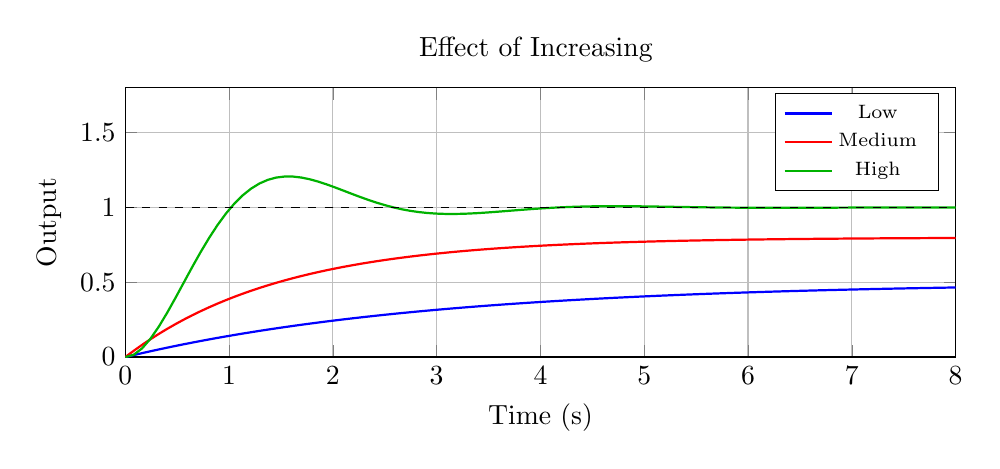
\begin{tikzpicture}
\begin{axis}[
    width=\textwidth,
    height=5cm,
    xlabel={Time (s)},
    ylabel={Output},
    xmin=0, xmax=8,
    ymin=0, ymax=1.8,
    title={Effect of Increasing $\Kp$},
    grid=major,
    legend style={font=\scriptsize, at={(0.98,0.98)}, anchor=north east}
]
\addplot[thick, blue, domain=0:8, samples=100]
    {0.5*(1 - exp(-x/3))};
\addlegendentry{Low $\Kp$}
\addplot[thick, red, domain=0:8, samples=100]
    {0.8*(1 - exp(-x/1.5))};
\addlegendentry{Medium $\Kp$}
\addplot[thick, green!70!black, domain=0:8, samples=100]
    {1 - exp(-x)*(cos(deg(2*x)) + 0.5*sin(deg(2*x)))};
\addlegendentry{High $\Kp$}
\addplot[dashed, black, domain=0:8] {1};
\end{axis}
\end{tikzpicture}
\end{subfigure}
\hfill
\begin{subfigure}[b]{0.48\textwidth}
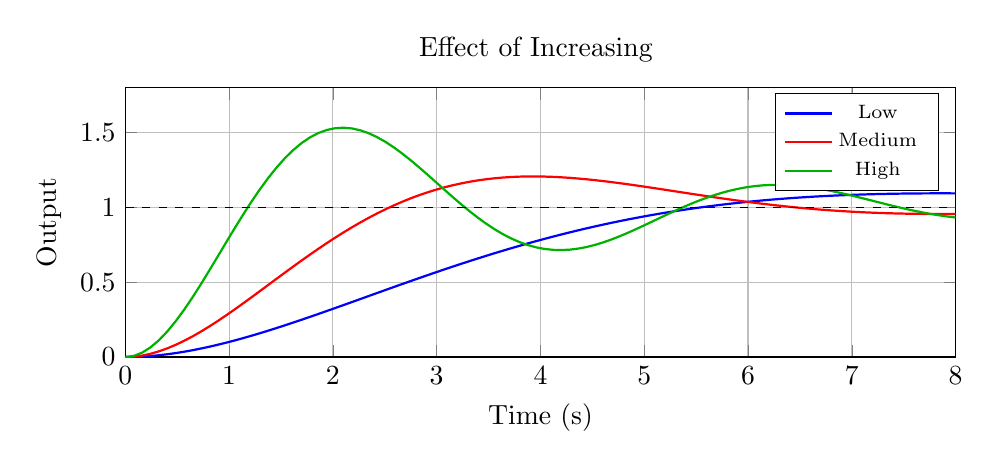
\begin{tikzpicture}
\begin{axis}[
    width=\textwidth,
    height=5cm,
    xlabel={Time (s)},
    ylabel={Output},
    xmin=0, xmax=8,
    ymin=0, ymax=1.8,
    title={Effect of Increasing $\Ki$},
    grid=major,
    legend style={font=\scriptsize, at={(0.98,0.98)}, anchor=north east}
]
\addplot[thick, blue, domain=0:8, samples=100]
    {1 - exp(-0.3*x)*(cos(deg(0.4*x)) + 0.75*sin(deg(0.4*x)))};
\addlegendentry{Low $\Ki$}
\addplot[thick, red, domain=0:8, samples=100]
    {1 - exp(-0.4*x)*(cos(deg(0.8*x)) + 0.5*sin(deg(0.8*x)))};
\addlegendentry{Medium $\Ki$}
\addplot[thick, green!70!black, domain=0:8, samples=100]
    {1 - exp(-0.3*x)*(cos(deg(1.5*x)) + 0.2*sin(deg(1.5*x)))};
\addlegendentry{High $\Ki$}
\addplot[dashed, black, domain=0:8] {1};
\end{axis}
\end{tikzpicture}
\end{subfigure}

\vspace{1em}

\begin{subfigure}[b]{0.48\textwidth}
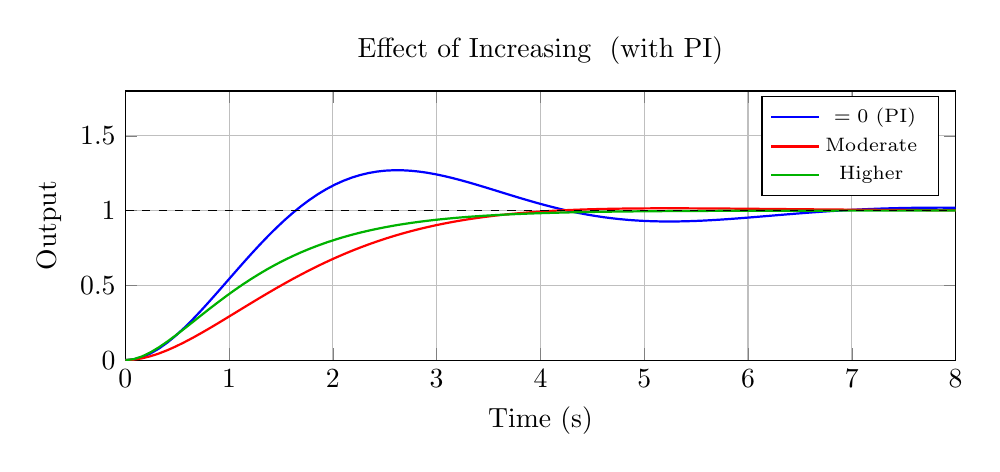
\begin{tikzpicture}
\begin{axis}[
    width=\textwidth,
    height=5cm,
    xlabel={Time (s)},
    ylabel={Output},
    xmin=0, xmax=8,
    ymin=0, ymax=1.8,
    title={Effect of Increasing $\Kd$ (with PI)},
    grid=major,
    legend style={font=\scriptsize, at={(0.98,0.98)}, anchor=north east}
]
\addplot[thick, blue, domain=0:8, samples=100]
    {1 - exp(-0.5*x)*(cos(deg(1.2*x)) + 0.42*sin(deg(1.2*x)))};
\addlegendentry{$\Kd = 0$ (PI)}
\addplot[thick, red, domain=0:8, samples=100]
    {1 - exp(-0.8*x)*(cos(deg(0.6*x)) + 1.33*sin(deg(0.6*x)))};
\addlegendentry{Moderate $\Kd$}
\addplot[thick, green!70!black, domain=0:8, samples=100]
    {1 - exp(-1.5*x)*(1 + 1.5*x)};
\addlegendentry{Higher $\Kd$}
\addplot[dashed, black, domain=0:8] {1};
\end{axis}
\end{tikzpicture}
\end{subfigure}
\caption{Effect of individually increasing each PID gain. (Top left) Increasing $\Kp$: faster rise but more overshoot and persistent offset. (Top right) Increasing $\Ki$: eliminates steady-state error but increases oscillation. (Bottom) Increasing $\Kd$: reduces overshoot and settling time.}
\label{fig:gain_effects}
\end{figure}

\subsection{Practical Controller Forms}

Not all applications require all three terms. Table~\ref{tab:controller_forms} summarizes the common reduced-order controllers and their typical applications.

\begin{table}[htbp]
\centering
\caption{Comparison of Practical Controller Forms}
\label{tab:controller_forms}
\begin{tabular}{lp{4cm}p{4.5cm}p{4cm}}
\toprule
\textbf{Type} & \textbf{Transfer Function} & \textbf{Characteristics} & \textbf{Applications} \\
\midrule
P & $C(s) = \Kp$ & Simplest form; used when steady-state error is acceptable & Non-critical level control, manual-like operation \\
\addlinespace
PI & $C(s) = \Kp + \dfrac{\Ki}{s}$ & Most common industrial controller; eliminates steady-state error without noise amplification & Flow control, pressure control, slow temperature loops \\
\addlinespace
PD & $C(s) = \Kp + \Kd s$ & Improves transient response without affecting steady-state; rarely used alone due to steady-state error & Systems where overshoot is critical and error is tolerable \\
\addlinespace
PID & Full three-term controller & Used when both steady-state accuracy and fast transient response are required & Precise temperature control, position control, process control \\
\bottomrule
\end{tabular}
\end{table}


%=============================================================================
\section{Practical Experiment: Temperature Control System}
%=============================================================================

Theory comes alive through hands-on experimentation. In this section, we design, build, and tune a PID temperature controller using readily available components. This experiment demonstrates the progressive improvement from P-only to PI to full PID control.

\subsection{System Overview}

Our experimental setup controls the temperature of a small thermal mass (an aluminum block or water bath) using a resistive heating element. The system uses an Arduino Uno (or compatible) \textbf{microcontroller} to read a 10k$\Omega$ NTC \textbf{thermistor} (or TMP36 analog sensor) for temperature sensing. A 10$\Omega$, 10W power resistor serves as the \textbf{heating element}, driven by an N-channel \textbf{MOSFET} (e.g., IRF520) for PWM control. The \textbf{thermal mass} consists of a small aluminum block (approximately $30 \times 30 \times 10$ mm), and the system is powered by a 12V, 2A DC \textbf{power supply}.

\begin{figure}[htbp]
\centering
\begin{circuitikz}[scale=0.9]
    % Arduino
    \draw[thick, fill=blue!10] (0,0) rectangle (3,4);
    \node at (1.5,3.5) {\textbf{Arduino}};
    \node at (1.5,2.5) {Uno};

    % Pin labels
    \node[right] at (3,1) {\scriptsize A0};
    \node[right] at (3,2) {\scriptsize D9};
    \node[right] at (3,3) {\scriptsize 5V};
    \node[right] at (3,0.3) {\scriptsize GND};

    % Thermistor circuit
    \draw (3,3) -- (5,3);
    \draw (5,3) to[R, l=$10k\Omega$] (5,1.5);
    \draw (5,1.5) to[thR, l_=NTC] (5,0);
    \draw (3,0.3) -- (5,0.3) -- (5,0);

    % Connection to A0
    \draw (5,1.5) -- (6,1.5) -- (6,1) -- (3.5,1) -- (3,1);
    \node[above] at (5.5,1.5) {\scriptsize $V_{temp}$};

    % MOSFET driver
    \draw (3,2) -- (8,2);
    \draw (8,2) to[R, l=\scriptsize $220\Omega$] (10,2);

    % MOSFET symbol
    \draw (10,2) -- (10.5,2);
    \draw (10.5,1) -- (10.5,3);
    \draw (10.5,1) -- (11,1) -- (11,0.5);
    \draw (10.5,3) -- (11,3) -- (11,3.5);
    \draw (10.5,2) -- (11,2);
    \draw (11,0.5) -- (11.5,0.5) -- (11.5,3.5) -- (11,3.5);
    \node[right] at (11.5,2) {\scriptsize MOSFET};

    % Heating element
    \draw (11.5,3.5) -- (11.5,5) -- (14,5);
    \draw (14,5) to[R, l=$10\Omega$] (14,2);
    \node[right] at (14.5,3.5) {\scriptsize Heater};

    % Power supply
    \draw (14,2) -- (14,0.5) -- (11.5,0.5);
    \draw (11.5,0.5) -- (5,0.5) -- (5,0.3);

    \draw (11.5,5) -- (11.5,5.5);
    \node[above] at (11.5,5.5) {+12V};

    % Thermal mass (aluminum block)
    \draw[thick, fill=gray!30] (13,1) rectangle (15.5,4);
    \node at (14.25,2.5) {\scriptsize Al block};

    % Thermistor attached to block
    \draw[dashed] (5,0.5) -- (5,-0.5) -- (13.5,-0.5) -- (13.5,1);
    \node[below] at (9,-0.5) {\scriptsize thermistor lead};

\end{circuitikz}
\caption{Wiring diagram for the PID temperature control experiment. The thermistor forms a voltage divider with a fixed resistor. The Arduino reads temperature via A0 and outputs PWM on D9 to control the MOSFET, which switches the heating element.}
\label{fig:wiring_diagram}
\end{figure}

\subsection{Software Implementation}

The following pseudocode implements P, PI, and PID control with selectable modes. Algorithm~\ref{alg:pid_init} shows the initialization procedure, Algorithm~\ref{alg:temp_read} presents the temperature reading function, and Algorithm~\ref{alg:pid_compute} details the core PID computation.

\begin{algorithm}[htbp]
\caption{PID Controller Initialization}
\label{alg:pid_init}
\begin{algorithmic}[1]
\State \textbf{Constants:} $R_{\text{series}} \gets 10000$, $R_{\text{nominal}} \gets 10000$, $T_{\text{nominal}} \gets 25$, $B \gets 3950$
\State \textbf{Gains:} $K_p \gets 50$, $K_i \gets 0.5$, $K_d \gets 10$
\State \textbf{Setpoint:} $T_{\text{setpoint}} \gets 50$ \Comment{Target temperature in Celsius}
\State \textbf{Mode:} $\text{controlMode} \gets 2$ \Comment{0 = P, 1 = PI, 2 = PID}
\State \textbf{State variables:} $\text{integral} \gets 0$, $e_{\text{prev}} \gets 0$, $t_{\text{prev}} \gets \Call{CurrentTime}{}$
\State \textbf{Anti-windup limit:} $I_{\text{max}} \gets 500$
\State Configure heater pin as output
\State Initialize serial communication for data logging
\end{algorithmic}
\end{algorithm}

\begin{algorithm}[htbp]
\caption{Temperature Reading from Thermistor}
\label{alg:temp_read}
\begin{algorithmic}[1]
\Require ADC reading from thermistor voltage divider
\Ensure Temperature in degrees Celsius
\State $V_{\text{raw}} \gets \Call{ReadADC}{\text{thermistor\_pin}}$
\State $R_{\text{thermistor}} \gets R_{\text{series}} / (1023 / V_{\text{raw}} - 1)$ \Comment{Voltage divider equation}
\State $x \gets \ln(R_{\text{thermistor}} / R_{\text{nominal}}) / B$ \Comment{Steinhart-Hart B-parameter model}
\State $x \gets x + 1 / (T_{\text{nominal}} + 273.15)$
\State $T_{\text{kelvin}} \gets 1 / x$
\State \Return $T_{\text{kelvin}} - 273.15$ \Comment{Convert to Celsius}
\end{algorithmic}
\end{algorithm}

\begin{algorithm}[htbp]
\caption{PID Control Computation}
\label{alg:pid_compute}
\begin{algorithmic}[1]
\Require Current temperature $T$, control mode, gains $(K_p, K_i, K_d)$
\Ensure Control output $u$ (PWM value 0--255)
\State $t_{\text{current}} \gets \Call{CurrentTime}{}$
\State $\Delta t \gets (t_{\text{current}} - t_{\text{prev}}) / 1000$ \Comment{Time step in seconds}
\If{$\Delta t \leq 0$}
    \State \Return 0
\EndIf
\State $e \gets T_{\text{setpoint}} - T$ \Comment{Calculate error}
\State $P \gets K_p \cdot e$ \Comment{Proportional term}
\State $I \gets 0$
\If{$\text{controlMode} \geq 1$} \Comment{Include integral action}
    \State $\text{integral} \gets \text{integral} + e \cdot \Delta t$
    \State $\text{integral} \gets \Call{Clamp}{\text{integral}, -I_{\text{max}}, I_{\text{max}}}$ \Comment{Anti-windup}
    \State $I \gets K_i \cdot \text{integral}$
\EndIf
\State $D \gets 0$
\If{$\text{controlMode} \geq 2$} \Comment{Include derivative action}
    \State $\dot{e} \gets (e - e_{\text{prev}}) / \Delta t$
    \State $D \gets K_d \cdot \dot{e}$
\EndIf
\State $e_{\text{prev}} \gets e$, $t_{\text{prev}} \gets t_{\text{current}}$ \Comment{Update state}
\State $u \gets P + I + D$
\State $u \gets \Call{Clamp}{u, 0, 255}$ \Comment{Constrain to valid PWM range}
\State \Return $u$
\end{algorithmic}
\end{algorithm}

\begin{algorithm}[htbp]
\caption{PID Controller Main Loop}
\label{alg:pid_main}
\begin{algorithmic}[1]
\Loop
    \State $T \gets \Call{ReadTemperature}{}$ \Comment{Get current temperature}
    \State $u \gets \Call{ComputePID}{T}$ \Comment{Calculate control output}
    \State $\Call{SetHeaterPWM}{u}$ \Comment{Apply to actuator}
    \State $\Call{LogData}{t, T_{\text{setpoint}}, T, u, e}$ \Comment{Record for analysis}
    \State $\Call{Wait}{100\text{ ms}}$ \Comment{10 Hz control loop}
\EndLoop
\end{algorithmic}
\end{algorithm}

\subsection{Experimental Procedure}

\textbf{Step 1: Characterize the Open-Loop System.}
Before implementing control, you must understand your plant. Apply a constant PWM signal (e.g., 128 corresponding to 50\% duty cycle) and record temperature versus time. From this response, identify the time constant $\tau$ as the time required to reach 63.2\% of the final value, and determine the steady-state gain $K$ as the temperature rise per unit PWM input.

\textbf{Step 2: P-Only Control.}
Set the control mode to proportional-only operation. Start with a low proportional gain $\Kp$ (e.g., 10) and increase it gradually while observing the steady-state error (offset from setpoint). You will notice that higher $\Kp$ reduces the offset but never eliminates it entirely---this is the fundamental limitation of proportional control.

\textbf{Step 3: PI Control.}
Enable integral action by switching to PI control mode while keeping the $\Kp$ value from Step 2. Start with a small integral gain $\Ki$ (e.g., 0.1) and increase it gradually. Observe how the steady-state error approaches zero as the integral term accumulates. Be aware that too much integral gain causes overshoot and oscillation.

\textbf{Step 4: PID Control.}
Enable full PID control while retaining the $\Kp$ and $\Ki$ values from previous steps. Start with a small derivative gain $\Kd$ (e.g., 5) and increase it gradually. Observe the reduced overshoot and faster settling time that derivative action provides. Note that excessive derivative gain may cause high-frequency oscillation due to noise sensitivity.

\subsection{Expected Results}

Figure~\ref{fig:experimental_results} shows typical experimental results from this setup.

\begin{figure}[htbp]
\centering
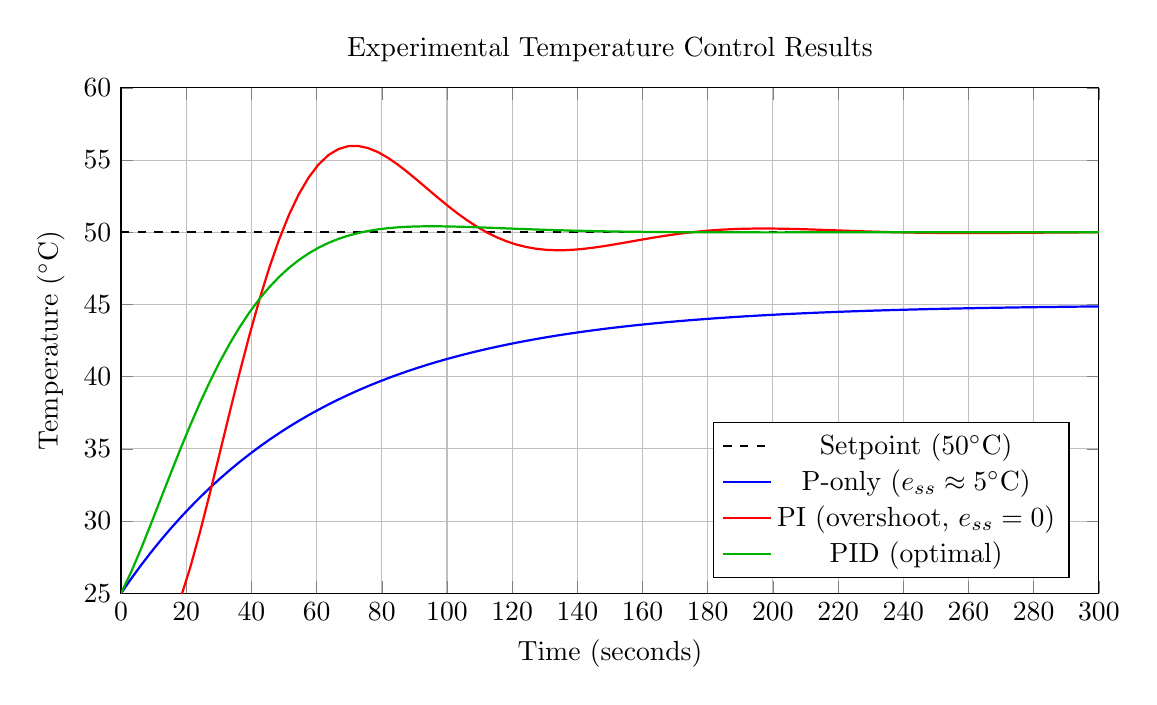
\begin{tikzpicture}
\begin{axis}[
    width=14cm,
    height=8cm,
    xlabel={Time (seconds)},
    ylabel={Temperature ($^\circ$C)},
    xmin=0, xmax=300,
    ymin=25, ymax=60,
    legend pos=south east,
    grid=major,
    title={Experimental Temperature Control Results}
]

% Setpoint
\addplot[thick, dashed, black, domain=0:300] {50};
\addlegendentry{Setpoint (50$^\circ$C)}

% P-only response (offset)
\addplot[thick, blue, domain=0:300, samples=100]
    {25 + 20*(1 - exp(-x/60))};
\addlegendentry{P-only ($e_{ss} \approx 5^\circ$C)}

% PI response (overshoot, zero error)
\addplot[thick, red, domain=0:300, samples=100]
    {25 + 25*(1 - exp(-x/40)*(cos(deg(0.05*x)) + 1.25*sin(deg(0.05*x))))};
\addlegendentry{PI (overshoot, $e_{ss} = 0$)}

% PID response (fast, accurate)
\addplot[thick, green!70!black, domain=0:300, samples=100]
    {25 + 25*(1 - exp(-x/25)*(cos(deg(0.03*x)) + 0.75*sin(deg(0.03*x))))};
\addlegendentry{PID (optimal)}

\end{axis}
\end{tikzpicture}
\caption{Typical experimental results from the temperature control experiment. P-only control reaches equilibrium quickly but with a 5$^\circ$C offset. PI control eliminates the offset but overshoots. PID control achieves fast settling with minimal overshoot.}
\label{fig:experimental_results}
\end{figure}


%=============================================================================
\section{Worked Examples}
%=============================================================================

This section provides detailed worked examples that reinforce the theoretical concepts and prepare students for practical controller design.

\begin{examplebox}[Steady-State Error with P-Only Control]
\label{ex:p_only_error}
A DC motor speed control system has the plant transfer function
\begin{equation*}
G(s) = \frac{10}{s + 2}
\end{equation*}
A proportional controller $C(s) = \Kp$ is used. Calculate the steady-state error to a unit step reference for $\Kp = 1, 5, 20$.

\textbf{Solution:}

The closed-loop transfer function is:
\begin{equation*}
T(s) = \frac{\Kp G(s)}{1 + \Kp G(s)} = \frac{\Kp \cdot \frac{10}{s+2}}{1 + \Kp \cdot \frac{10}{s+2}} = \frac{10\Kp}{s + 2 + 10\Kp}
\end{equation*}

The error transfer function is:
\begin{equation*}
\frac{E(s)}{R(s)} = 1 - T(s) = \frac{s + 2}{s + 2 + 10\Kp}
\end{equation*}

For a unit step input $R(s) = 1/s$, applying the final value theorem:
\begin{equation*}
e_{ss} = \lim_{s \to 0} s \cdot \frac{s + 2}{s + 2 + 10\Kp} \cdot \frac{1}{s} = \frac{2}{2 + 10\Kp}
\end{equation*}

Evaluating for each gain:
\begin{align*}
\Kp = 1: \quad e_{ss} &= \frac{2}{2 + 10} = \frac{2}{12} = 0.167 \quad (16.7\%) \\
\Kp = 5: \quad e_{ss} &= \frac{2}{2 + 50} = \frac{2}{52} = 0.038 \quad (3.8\%) \\
\Kp = 20: \quad e_{ss} &= \frac{2}{2 + 200} = \frac{2}{202} = 0.0099 \quad (0.99\%)
\end{align*}

\textbf{Observation:} Even with $\Kp = 20$, there is still nearly 1\% steady-state error. This can only be eliminated with integral action.
\end{examplebox}

\begin{examplebox}[Integral Action Eliminates Steady-State Error]
\label{ex:pi_zero_error}
For the same motor system as Example~\ref{ex:p_only_error}, show that a PI controller eliminates steady-state error.

\textbf{Solution:}

With a PI controller:
\begin{equation*}
C(s) = \Kp + \frac{\Ki}{s} = \frac{\Kp s + \Ki}{s}
\end{equation*}

The open-loop transfer function is:
\begin{equation*}
L(s) = C(s)G(s) = \frac{(\Kp s + \Ki)}{s} \cdot \frac{10}{s + 2} = \frac{10(\Kp s + \Ki)}{s(s + 2)}
\end{equation*}

The system is now Type 1 (one integrator in the open-loop). The error transfer function is:
\begin{equation*}
\frac{E(s)}{R(s)} = \frac{1}{1 + L(s)} = \frac{s(s+2)}{s(s+2) + 10(\Kp s + \Ki)}
\end{equation*}

For a unit step input, applying the final value theorem:
\begin{equation*}
e_{ss} = \lim_{s \to 0} s \cdot \frac{s(s+2)}{s(s+2) + 10(\Kp s + \Ki)} \cdot \frac{1}{s}
\end{equation*}

Evaluating the limit:
\begin{equation*}
e_{ss} = \lim_{s \to 0} \frac{s(s+2)}{s(s+2) + 10(\Kp s + \Ki)} = \frac{0 \cdot 2}{0 \cdot 2 + 10 \cdot \Ki} = \frac{0}{10\Ki} = 0
\end{equation*}

\textbf{Conclusion:} The integral action provides zero steady-state error for step inputs, regardless of the specific values of $\Kp$ and $\Ki$ (provided the closed-loop system is stable).
\end{examplebox}

\begin{example}[Effect of Derivative Action on Damping]
\label{ex:derivative_damping}
Consider a second-order plant:
\begin{equation*}
G(s) = \frac{1}{s^2 + 2s + 1}
\end{equation*}

Compare the closed-loop response with (a) P-only control ($\Kp = 10$) and (b) PD control ($\Kp = 10$, $\Kd = 2$).

\textbf{Solution:}

\textbf{(a) P-only control:}
\begin{equation*}
T(s) = \frac{10 \cdot \frac{1}{s^2 + 2s + 1}}{1 + 10 \cdot \frac{1}{s^2 + 2s + 1}} = \frac{10}{s^2 + 2s + 1 + 10} = \frac{10}{s^2 + 2s + 11}
\end{equation*}

The characteristic equation is $s^2 + 2s + 11 = 0$.

Poles: $s = \dfrac{-2 \pm \sqrt{4 - 44}}{2} = -1 \pm j\sqrt{10} \approx -1 \pm j3.16$

Natural frequency: $\omega_n = \sqrt{11} \approx 3.32$ rad/s

Damping ratio: $\zeta = \dfrac{2}{2\sqrt{11}} = \dfrac{1}{\sqrt{11}} \approx 0.30$

Overshoot: $M_p = e^{-\pi\zeta/\sqrt{1-\zeta^2}} \approx e^{-0.99} \approx 37\%$

\textbf{(b) PD control:}
\begin{equation*}
C(s) = 10 + 2s
\end{equation*}
\begin{equation*}
T(s) = \frac{(10 + 2s) \cdot \frac{1}{s^2 + 2s + 1}}{1 + (10 + 2s) \cdot \frac{1}{s^2 + 2s + 1}} = \frac{2s + 10}{s^2 + 2s + 1 + 2s + 10} = \frac{2s + 10}{s^2 + 4s + 11}
\end{equation*}

The characteristic equation is $s^2 + 4s + 11 = 0$.

Poles: $s = \dfrac{-4 \pm \sqrt{16 - 44}}{2} = -2 \pm j\sqrt{7} \approx -2 \pm j2.65$

Natural frequency: $\omega_n = \sqrt{11} \approx 3.32$ rad/s (unchanged)

Damping ratio: $\zeta = \dfrac{4}{2\sqrt{11}} = \dfrac{2}{\sqrt{11}} \approx 0.60$

Overshoot: $M_p = e^{-\pi\zeta/\sqrt{1-\zeta^2}} \approx e^{-2.36} \approx 9.5\%$

\textbf{Conclusion:} The derivative action doubled the damping ratio (from 0.30 to 0.60) and reduced overshoot from 37\% to 9.5\%. The natural frequency remained unchanged, but the system settles much faster due to the increased damping.
\end{example}

\begin{example}[PI Controller Design for Specified Error]
\label{ex:pi_design}
Design a PI controller for the plant
\begin{equation*}
G(s) = \frac{5}{s + 1}
\end{equation*}
such that the closed-loop system has zero steady-state error to step inputs and a phase margin of at least 60°.

\textbf{Solution:}

The PI controller in standard form is:
\begin{equation*}
C(s) = \Kp\left(1 + \frac{1}{\Ti s}\right) = \Kp \cdot \frac{\Ti s + 1}{\Ti s}
\end{equation*}

The open-loop transfer function is:
\begin{equation*}
L(s) = C(s)G(s) = \Kp \cdot \frac{\Ti s + 1}{\Ti s} \cdot \frac{5}{s + 1} = \frac{5\Kp(\Ti s + 1)}{\Ti s(s + 1)}
\end{equation*}

\textbf{Step 1: Place the PI zero to cancel the plant pole.}

Setting $\Ti = 1$ cancels the pole at $s = -1$:
\begin{equation*}
L(s) = \frac{5\Kp(s + 1)}{s(s + 1)} = \frac{5\Kp}{s}
\end{equation*}

\textbf{Step 2: Design for phase margin.}

For $L(s) = 5\Kp/s$, the phase is $\angle L(j\omega) = -90°$ for all $\omega$, giving a phase margin of $PM = 180° - 90° = 90°$, which satisfies the requirement.

At the gain crossover frequency $\omega_{gc}$:
\begin{equation*}
|L(j\omega_{gc})| = 1 \implies \frac{5\Kp}{\omega_{gc}} = 1 \implies \omega_{gc} = 5\Kp
\end{equation*}

For reasonable bandwidth (say, $\omega_{gc} = 5$ rad/s), we choose $\Kp = 1$.

\textbf{Final Design:}
\begin{equation*}
\boxed{C(s) = 1 + \frac{1}{s} = \frac{s + 1}{s}}
\end{equation*}

Verification confirms that the steady-state error is zero (Type 1 system), the phase margin of 90° exceeds the 60° requirement, and the gain crossover frequency is 5 rad/s.
\end{example}

\begin{example}[Closed-Loop Stability Analysis with PID]
\label{ex:stability_analysis}
Determine the range of $\Kp$ for which the following PID-controlled system is stable:
\begin{align*}
\text{Plant:} \quad G(s) &= \frac{1}{s(s+1)(s+2)} \\
\text{Controller:} \quad C(s) &= \Kp + \frac{0.5}{s} + 0.5s
\end{align*}

\textbf{Solution:}

The controller transfer function is:
\begin{equation*}
C(s) = \Kp + \frac{0.5}{s} + 0.5s = \frac{0.5s^2 + \Kp s + 0.5}{s} = \frac{0.5(s^2 + 2\Kp s + 1)}{s}
\end{equation*}

The characteristic equation of the closed-loop system is:
\begin{equation*}
1 + C(s)G(s) = 0
\end{equation*}

\begin{equation*}
1 + \frac{0.5(s^2 + 2\Kp s + 1)}{s} \cdot \frac{1}{s(s+1)(s+2)} = 0
\end{equation*}

Multiplying through:
\begin{equation*}
s^2(s+1)(s+2) + 0.5(s^2 + 2\Kp s + 1) = 0
\end{equation*}

Expanding:
\begin{equation*}
s^2(s^2 + 3s + 2) + 0.5s^2 + \Kp s + 0.5 = 0
\end{equation*}
\begin{equation*}
s^4 + 3s^3 + 2s^2 + 0.5s^2 + \Kp s + 0.5 = 0
\end{equation*}
\begin{equation*}
s^4 + 3s^3 + 2.5s^2 + \Kp s + 0.5 = 0
\end{equation*}

\textbf{Routh Array:}
\begin{center}
\begin{tabular}{c|cc}
$s^4$ & 1 & 2.5 \\
$s^3$ & 3 & $\Kp$ \\
$s^2$ & $\dfrac{7.5 - \Kp}{3}$ & 0.5 \\
$s^1$ & $\dfrac{(7.5-\Kp)\Kp - 4.5}{7.5 - \Kp}$ & 0 \\
$s^0$ & 0.5 & \\
\end{tabular}
\end{center}

For stability, all first-column elements must be positive:

\textbf{Condition 1:} $\dfrac{7.5 - \Kp}{3} > 0 \implies \Kp < 7.5$

\textbf{Condition 2:} $\dfrac{(7.5-\Kp)\Kp - 4.5}{7.5 - \Kp} > 0$

Since $\Kp < 7.5$, the denominator is positive, so we need:
\begin{equation*}
(7.5 - \Kp)\Kp - 4.5 > 0
\end{equation*}
\begin{equation*}
-\Kp^2 + 7.5\Kp - 4.5 > 0
\end{equation*}
\begin{equation*}
\Kp^2 - 7.5\Kp + 4.5 < 0
\end{equation*}

Using the quadratic formula:
\begin{equation*}
\Kp = \frac{7.5 \pm \sqrt{56.25 - 18}}{2} = \frac{7.5 \pm \sqrt{38.25}}{2} = \frac{7.5 \pm 6.18}{2}
\end{equation*}

So $\Kp \in (0.66, 6.84)$

Combined with Condition 1: $\boxed{0.66 < \Kp < 6.84}$

\textbf{Conclusion:} The PID-controlled system is stable for $0.66 < \Kp < 6.84$. Outside this range, the system becomes unstable.
\end{example}

\begin{example}[Digital PID Implementation Considerations]
\label{ex:digital_pid}
A continuous-time PID controller has parameters $\Kp = 2$, $\Ti = 4$ s, $\Td = 0.5$ s. Derive the discrete-time difference equation for implementation with sampling period $T_s = 0.1$ s.

\textbf{Solution:}

The continuous-time PID in standard form is:
\begin{equation*}
u(t) = \Kp \left[ e(t) + \frac{1}{\Ti} \int_0^t e(\tau) d\tau + \Td \frac{de(t)}{dt} \right]
\end{equation*}

\textbf{Discretization:}

\textit{Proportional term:} Direct sampling
\begin{equation*}
P[k] = \Kp \cdot e[k]
\end{equation*}

\textit{Integral term:} Backward Euler (rectangular) approximation
\begin{equation*}
I[k] = I[k-1] + \frac{\Kp T_s}{\Ti} e[k]
\end{equation*}

\textit{Derivative term:} Backward difference
\begin{equation*}
D[k] = \frac{\Kp \Td}{T_s} (e[k] - e[k-1])
\end{equation*}

\textbf{Complete discrete PID:}
\begin{equation*}
u[k] = P[k] + I[k] + D[k]
\end{equation*}

\textbf{Numerical values:}

With $\Kp = 2$, $\Ti = 4$, $\Td = 0.5$, $T_s = 0.1$:
\begin{align*}
P[k] &= 2 \cdot e[k] \\
I[k] &= I[k-1] + \frac{2 \times 0.1}{4} e[k] = I[k-1] + 0.05 \cdot e[k] \\
D[k] &= \frac{2 \times 0.5}{0.1} (e[k] - e[k-1]) = 10 \cdot (e[k] - e[k-1])
\end{align*}

\textbf{Velocity form} (for anti-windup):
\begin{equation*}
\Delta u[k] = u[k] - u[k-1] = \Kp\left[(e[k]-e[k-1]) + \frac{T_s}{\Ti}e[k] + \frac{\Td}{T_s}(e[k] - 2e[k-1] + e[k-2])\right]
\end{equation*}

This incremental form is preferred in practice because it automatically handles integral windup when the output saturates.
\end{example}


%=============================================================================
\section{Chapter Summary}
%=============================================================================

This chapter has provided a comprehensive treatment of PID control, from its historical origins to modern implementation.

Regarding \textbf{historical development}, PID control evolved from practical ship steering problems (Sperry, 1911) through rigorous theoretical analysis (Minorsky, 1922) to widespread industrial adoption via pneumatic controllers (1930s--1940s).

The \textbf{PID control law} is expressed mathematically as:
\begin{equation*}
u(t) = \Kp e(t) + \Ki \int_0^t e(\tau) d\tau + \Kd \frac{de(t)}{dt}
\end{equation*}

Understanding the \textbf{role of each term} is essential. The proportional term provides fast response but cannot eliminate steady-state error. The integral term eliminates steady-state error but may cause overshoot. The derivative term provides damping and anticipation but amplifies noise.

From a \textbf{practical standpoint}, derivative filtering, anti-windup, and digital implementation are essential for real-world applications.

Finally, \textbf{PID dominance} in industry is explained by the combination of simplicity, robustness, and versatility, which is why PID controllers constitute over 90\% of all industrial control loops.


\newpage
%=============================================================================
\section{Exercises}
%=============================================================================

\begin{exercise}
A temperature control system has plant transfer function $G(s) = \dfrac{2}{5s + 1}$. Design a PI controller such that the closed-loop system has a damping ratio of 0.7 and zero steady-state error to step inputs.
\end{exercise}

\begin{exercise}
For the system in Exercise 1, add derivative action to achieve a settling time of less than 3 seconds while maintaining zero steady-state error.
\end{exercise}

\begin{exercise}
Prove that a Type 0 plant with P-only control always has non-zero steady-state error for step inputs, regardless of the proportional gain value.
\end{exercise}

\begin{exercise}
A quadrotor altitude controller uses the transfer function $G(s) = \dfrac{1}{s^2}$ (double integrator). Explain why P-only control is marginally stable and design a PD controller for stable operation with damping ratio $\zeta = 0.707$.
\end{exercise}

\begin{exercise}
Using the Routh-Hurwitz criterion, determine the range of $\Ki$ for which the PI-controlled system with $G(s) = \dfrac{1}{s(s+1)(s+3)}$ and $\Kp = 2$ is stable.
\end{exercise}

\begin{exercise}
Implement a digital PID controller for an Arduino-based motor speed control system. The sampling rate is 100 Hz, and the desired response should have no more than 10\% overshoot with settling time under 0.5 seconds. Document your tuning procedure.
\end{exercise}

\begin{exercise}
Research and explain three different anti-windup strategies for integral action. Compare their effectiveness for systems with significant actuator saturation.
\end{exercise}

\begin{exercise}
The Ziegler-Nichols tuning method (covered in Chapter 11) provides initial PID gains based on critical gain and period. For a system with critical gain $K_u = 10$ and critical period $T_u = 2$ s, calculate the Ziegler-Nichols PID parameters and discuss their expected performance characteristics.
\end{exercise}

\begin{exercise}
Consider a liquid level control system with plant $G(s) = \dfrac{1}{s(s+1)}$. Design a PID controller to achieve zero steady-state error for step inputs while maintaining a phase margin of at least 45 degrees. Verify your design using Bode plot analysis.
\end{exercise}

\begin{exercise}
Explain the physical interpretation of each PID term (proportional, integral, derivative) in the context of automotive cruise control. Why might derivative action be problematic in this application?
\end{exercise}

\begin{exercise}
A servo motor position control system has the transfer function $G(s) = \dfrac{100}{s(s+10)}$. Compare the step response characteristics (rise time, overshoot, settling time) for P, PI, and PID controllers with appropriately tuned gains.
\end{exercise}

\begin{exercise}
Derive the transfer function of an ideal PID controller in the frequency domain and explain how each term affects the Bode magnitude and phase plots.
\end{exercise}


%=============================================================================
% References
%=============================================================================

\begin{thebibliography}{9}

\bibitem{minorsky1922}
N. Minorsky, ``Directional stability of automatically steered bodies,''
\textit{Journal of the American Society of Naval Engineers}, vol. 34, no. 2, pp. 280--309, 1922.

\bibitem{astrom2006}
K. J. \r{A}str\"om and T. H\"agglund, \textit{Advanced PID Control}.
Research Triangle Park, NC: ISA, 2006.

\bibitem{bennett1993}
S. Bennett, ``Development of the PID controller,''
\textit{IEEE Control Systems Magazine}, vol. 13, no. 6, pp. 58--62, Dec. 1993.

\bibitem{ziegler1942}
J. G. Ziegler and N. B. Nichols, ``Optimum settings for automatic controllers,''
\textit{Transactions of the ASME}, vol. 64, pp. 759--768, 1942.

\bibitem{sperry1913}
E. A. Sperry, ``The gyroscope for marine purposes,''
\textit{Transactions of the Society of Naval Architects and Marine Engineers}, vol. 21, pp. 203--252, 1913.

\bibitem{ogata2010}
K. Ogata, \textit{Modern Control Engineering}, 5th ed.
Upper Saddle River, NJ: Prentice Hall, 2010.

\bibitem{seborg2011}
D. E. Seborg, T. F. Edgar, D. A. Mellichamp, and F. J. Doyle III,
\textit{Process Dynamics and Control}, 3rd ed.
Hoboken, NJ: Wiley, 2011.

\end{thebibliography}


